\section{A Integral}

\subsection*{Um pouco de história}

\begin{frame}[label=area-circulo]{A origem do Cálculo Integral}
	Na segunda metade do século XVII, \textcolor{blue}{Newton} na Inglaterra e \textcolor{blue}{Leibniz} na Alemanha mudaram o curso da matemática para sempre. Ele pegaram uma colcha de retalhos soltas de ideias sobre movimento e curvas e transformaram isso no cálculo. 


	\begin{center}
				\begin{minipage}{0.4\textwidth}
\begin{center}
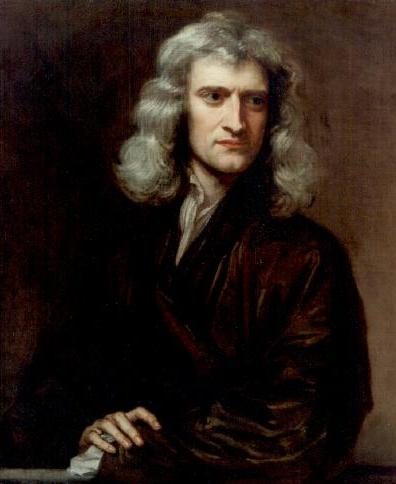
\includegraphics[scale=0.35]{newton.jpg}

{\scriptsize 	Isaac Newton\\ 1643-1727 }
\end{center}
	\end{minipage}	
	\begin{minipage}{0.4\textwidth}
		
\begin{center}
	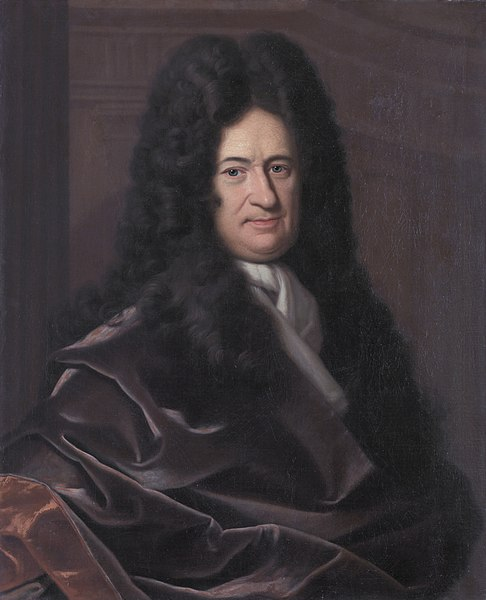
\includegraphics[scale=0.2]{leibniz.jpg}

			{\scriptsize Gottfried Wilhelm Leibniz \\  1646-1716 }
\end{center}
	\end{minipage}
	\end{center}
\end{frame}



\begin{frame}[label=area-circulo]{O Precursor do Cálculo}
	Muitos historiadores acreditam que  o verdadeiro precursor do cálculo foi \textcolor{blue}{Arquimedes}. Ele aperfeiçoou o método da exaustão de Eudoxus para  encontrar áreas de figuras planas. 
\medskip

Arquimedes é considerado o maior matemático da antiguidade. Segundo a lenda, foi morto por um soldado romano durante a tomada da cidade enquanto estudava um diagrama geométrico na areia.
\smallskip

	\begin{minipage}{0.3\linewidth}
		
	\begin{center}
		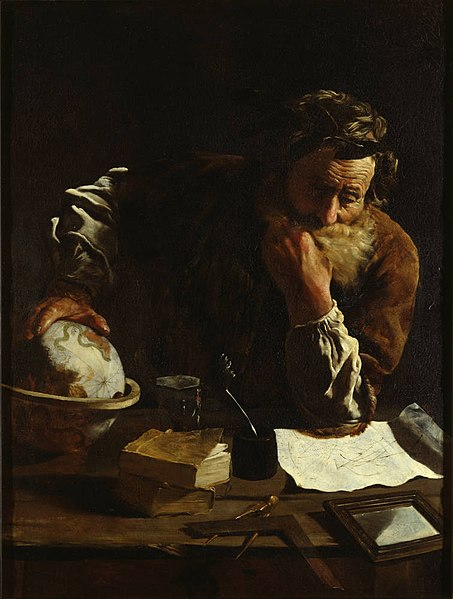
\includegraphics[scale=0.15]{arquimedes.jpg}
		
		{\tiny Arquimedes de Siracusa \\ 287-212 BCE. \\ Pint. Domenico Fetti (1620)}
	\end{center}
	
	\end{minipage}
\begin{minipage}{0.65\linewidth}
	 
	
	Em seu livro \textcolor{blue}{A Medida do Círculo} ele mostrou que o valor exato do número $\pi$   está entre \textcolor{red}{223/71 e 22/7}, ou seja, estaria aproximadamente entre \textcolor{red}{3,1408 e 3,1429}, aproximação que obteve inscrevendo e circunscrevendo o círculo em um polígono regular de \textcolor{red}{96 lados}. Usando este método ele foi capaz de calcular o volume da esfera, o volume e a área do cone, o volume obtido por revolução de qualquer segmento de uma parábola ou hipérbole.
\end{minipage}
\end{frame}


\begin{frame}[label=area-circulo]{Método da Exaustão de Eudoxus}


\begin{center}
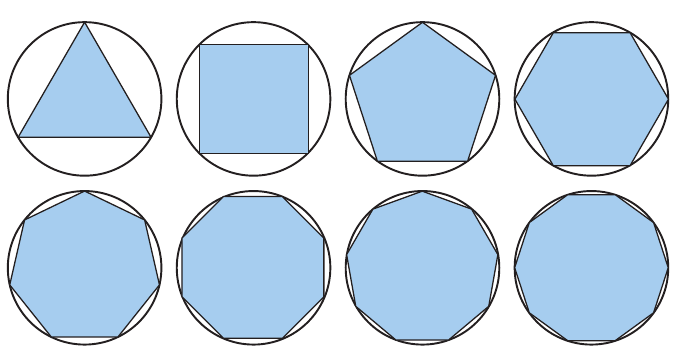
\includegraphics[scale=.5]{figuras/circulo-area.png}
\end{center}

\end{frame}

\begin{frame}[label=area-circulo,fragile=singleslide]{Polígonos Inscritos}
Na tabela abaixo temos a área $A_n$ de um polígono regular de $n$ lados inscrito em um círculo de raio 1.
\medskip

%	\begin{scriptsize}
\begin{center}
		\begin{pycode}
import sympy as sp

#dados iniciais
m=6 #começando com um hexágono regular
l=1 #lado do hexágono

#aproximação da área usando um polígono de n lados inscritos no círculo
print(r"\begin{tabular}{c|c|c}")
print(r" n &  $A_n$ & erro \\ \hline")
for n in range(10):
 h=sp.sqrt(1-l**2/4) #altura de cada triângulo dado o lado
 l=sp.sqrt(l**2/4+(1-h)**2) #lado do polígono da próxima iteração
 m=2*m  #número de lados do polígono seguinte  
 p=m*l  #perímetro do polígono de n lados 
 c=p/2
 n+=1
 print(r" ",m,"&",p/2,"&",sp.pi.evalf()-c,r"\\")
print(r"\end{tabular}")
		\end{pycode}
\end{center}
%	\end{scriptsize}
\end{frame}




\begin{frame}[label=area-circulo]{A ideia da integral}


\begin{center}
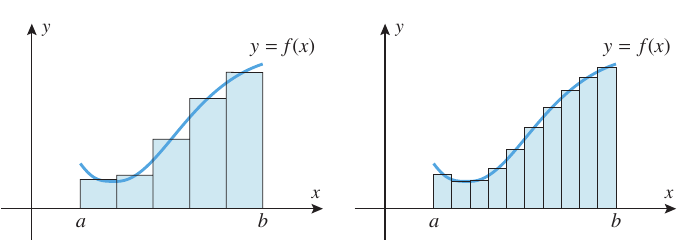
\includegraphics[scale=.55]{figuras/soma-rieman1.png}

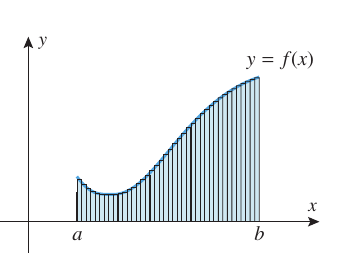
\includegraphics[scale=.55]{figuras/soma-rieman2.png}
\end{center}

\end{frame}


